% Options for packages loaded elsewhere
\PassOptionsToPackage{unicode}{hyperref}
\PassOptionsToPackage{hyphens}{url}
%
\documentclass[
]{article}
\usepackage{amsmath,amssymb}
\usepackage{lmodern}
\usepackage{ifxetex,ifluatex}
\ifnum 0\ifxetex 1\fi\ifluatex 1\fi=0 % if pdftex
  \usepackage[T1]{fontenc}
  \usepackage[utf8]{inputenc}
  \usepackage{textcomp} % provide euro and other symbols
\else % if luatex or xetex
  \usepackage{unicode-math}
  \defaultfontfeatures{Scale=MatchLowercase}
  \defaultfontfeatures[\rmfamily]{Ligatures=TeX,Scale=1}
\fi
% Use upquote if available, for straight quotes in verbatim environments
\IfFileExists{upquote.sty}{\usepackage{upquote}}{}
\IfFileExists{microtype.sty}{% use microtype if available
  \usepackage[]{microtype}
  \UseMicrotypeSet[protrusion]{basicmath} % disable protrusion for tt fonts
}{}
\makeatletter
\@ifundefined{KOMAClassName}{% if non-KOMA class
  \IfFileExists{parskip.sty}{%
    \usepackage{parskip}
  }{% else
    \setlength{\parindent}{0pt}
    \setlength{\parskip}{6pt plus 2pt minus 1pt}}
}{% if KOMA class
  \KOMAoptions{parskip=half}}
\makeatother
\usepackage{xcolor}
\IfFileExists{xurl.sty}{\usepackage{xurl}}{} % add URL line breaks if available
\IfFileExists{bookmark.sty}{\usepackage{bookmark}}{\usepackage{hyperref}}
\hypersetup{
  pdftitle={Teaching Data Science to Students in Biology using R, RStudio and Learnr: Analysis of Three years Data},
  hidelinks,
  pdfcreator={LaTeX via pandoc}}
\urlstyle{same} % disable monospaced font for URLs
\usepackage[margin=1in]{geometry}
\usepackage{color}
\usepackage{fancyvrb}
\newcommand{\VerbBar}{|}
\newcommand{\VERB}{\Verb[commandchars=\\\{\}]}
\DefineVerbatimEnvironment{Highlighting}{Verbatim}{commandchars=\\\{\}}
% Add ',fontsize=\small' for more characters per line
\usepackage{framed}
\definecolor{shadecolor}{RGB}{248,248,248}
\newenvironment{Shaded}{\begin{snugshade}}{\end{snugshade}}
\newcommand{\AlertTok}[1]{\textcolor[rgb]{0.94,0.16,0.16}{#1}}
\newcommand{\AnnotationTok}[1]{\textcolor[rgb]{0.56,0.35,0.01}{\textbf{\textit{#1}}}}
\newcommand{\AttributeTok}[1]{\textcolor[rgb]{0.77,0.63,0.00}{#1}}
\newcommand{\BaseNTok}[1]{\textcolor[rgb]{0.00,0.00,0.81}{#1}}
\newcommand{\BuiltInTok}[1]{#1}
\newcommand{\CharTok}[1]{\textcolor[rgb]{0.31,0.60,0.02}{#1}}
\newcommand{\CommentTok}[1]{\textcolor[rgb]{0.56,0.35,0.01}{\textit{#1}}}
\newcommand{\CommentVarTok}[1]{\textcolor[rgb]{0.56,0.35,0.01}{\textbf{\textit{#1}}}}
\newcommand{\ConstantTok}[1]{\textcolor[rgb]{0.00,0.00,0.00}{#1}}
\newcommand{\ControlFlowTok}[1]{\textcolor[rgb]{0.13,0.29,0.53}{\textbf{#1}}}
\newcommand{\DataTypeTok}[1]{\textcolor[rgb]{0.13,0.29,0.53}{#1}}
\newcommand{\DecValTok}[1]{\textcolor[rgb]{0.00,0.00,0.81}{#1}}
\newcommand{\DocumentationTok}[1]{\textcolor[rgb]{0.56,0.35,0.01}{\textbf{\textit{#1}}}}
\newcommand{\ErrorTok}[1]{\textcolor[rgb]{0.64,0.00,0.00}{\textbf{#1}}}
\newcommand{\ExtensionTok}[1]{#1}
\newcommand{\FloatTok}[1]{\textcolor[rgb]{0.00,0.00,0.81}{#1}}
\newcommand{\FunctionTok}[1]{\textcolor[rgb]{0.00,0.00,0.00}{#1}}
\newcommand{\ImportTok}[1]{#1}
\newcommand{\InformationTok}[1]{\textcolor[rgb]{0.56,0.35,0.01}{\textbf{\textit{#1}}}}
\newcommand{\KeywordTok}[1]{\textcolor[rgb]{0.13,0.29,0.53}{\textbf{#1}}}
\newcommand{\NormalTok}[1]{#1}
\newcommand{\OperatorTok}[1]{\textcolor[rgb]{0.81,0.36,0.00}{\textbf{#1}}}
\newcommand{\OtherTok}[1]{\textcolor[rgb]{0.56,0.35,0.01}{#1}}
\newcommand{\PreprocessorTok}[1]{\textcolor[rgb]{0.56,0.35,0.01}{\textit{#1}}}
\newcommand{\RegionMarkerTok}[1]{#1}
\newcommand{\SpecialCharTok}[1]{\textcolor[rgb]{0.00,0.00,0.00}{#1}}
\newcommand{\SpecialStringTok}[1]{\textcolor[rgb]{0.31,0.60,0.02}{#1}}
\newcommand{\StringTok}[1]{\textcolor[rgb]{0.31,0.60,0.02}{#1}}
\newcommand{\VariableTok}[1]{\textcolor[rgb]{0.00,0.00,0.00}{#1}}
\newcommand{\VerbatimStringTok}[1]{\textcolor[rgb]{0.31,0.60,0.02}{#1}}
\newcommand{\WarningTok}[1]{\textcolor[rgb]{0.56,0.35,0.01}{\textbf{\textit{#1}}}}
\usepackage{longtable,booktabs,array}
\usepackage{calc} % for calculating minipage widths
% Correct order of tables after \paragraph or \subparagraph
\usepackage{etoolbox}
\makeatletter
\patchcmd\longtable{\par}{\if@noskipsec\mbox{}\fi\par}{}{}
\makeatother
% Allow footnotes in longtable head/foot
\IfFileExists{footnotehyper.sty}{\usepackage{footnotehyper}}{\usepackage{footnote}}
\makesavenoteenv{longtable}
\usepackage{graphicx}
\makeatletter
\def\maxwidth{\ifdim\Gin@nat@width>\linewidth\linewidth\else\Gin@nat@width\fi}
\def\maxheight{\ifdim\Gin@nat@height>\textheight\textheight\else\Gin@nat@height\fi}
\makeatother
% Scale images if necessary, so that they will not overflow the page
% margins by default, and it is still possible to overwrite the defaults
% using explicit options in \includegraphics[width, height, ...]{}
\setkeys{Gin}{width=\maxwidth,height=\maxheight,keepaspectratio}
% Set default figure placement to htbp
\makeatletter
\def\fps@figure{htbp}
\makeatother
\setlength{\emergencystretch}{3em} % prevent overfull lines
\providecommand{\tightlist}{%
  \setlength{\itemsep}{0pt}\setlength{\parskip}{0pt}}
\setcounter{secnumdepth}{5}
\ifluatex
  \usepackage{selnolig}  % disable illegal ligatures
\fi
\newlength{\cslhangindent}
\setlength{\cslhangindent}{1.5em}
\newlength{\csllabelwidth}
\setlength{\csllabelwidth}{3em}
\newenvironment{CSLReferences}[2] % #1 hanging-ident, #2 entry spacing
 {% don't indent paragraphs
  \setlength{\parindent}{0pt}
  % turn on hanging indent if param 1 is 1
  \ifodd #1 \everypar{\setlength{\hangindent}{\cslhangindent}}\ignorespaces\fi
  % set entry spacing
  \ifnum #2 > 0
  \setlength{\parskip}{#2\baselineskip}
  \fi
 }%
 {}
\usepackage{calc}
\newcommand{\CSLBlock}[1]{#1\hfill\break}
\newcommand{\CSLLeftMargin}[1]{\parbox[t]{\csllabelwidth}{#1}}
\newcommand{\CSLRightInline}[1]{\parbox[t]{\linewidth - \csllabelwidth}{#1}\break}
\newcommand{\CSLIndent}[1]{\hspace{\cslhangindent}#1}

\title{Teaching Data Science to Students in Biology using R, RStudio and
Learnr: Analysis of Three years Data}
\author{}
\date{\vspace{-2.5em}}

\begin{document}
\maketitle

\hypertarget{abstract}{%
\section{Abstract}\label{abstract}}

\textbf{This is the original abstract that should be reworked according
to final content of the manuscript.}

The courses in biostatistics in biology at the University of Mons,
Belgium, were completely refactored in 2018 into data science courses
(see \url{http://bds.sciviews.org}). The content is expanded beyond
statistics to include computing tools, version management, reproducible
analyses, critical thinking and open data. Flipped classroom approach is
used. Students learn with the online material and they apply the
concepts on individual and group projects using a preconfigured virtual
machine with R and RStudio. Activities (H5P, learnr or Shiny
applications) are recorded in a MongoDB database (300,000+ events for
180+ students and 2,000+ GitHub repositories at
\url{https://github.com/BioDataScience-Course}). The analysis of these
data reveals several trends. (1) There is a relatively long lag period
required for the students to get used to the computing environment, the
teaching method and the data science in general. (2) Implication is very
high, with more than 85\% of the students that complete all the
activities and got good to excellent assessment. (3) There is a gap
between students' own perception of their skills achievements and their
assessment results: they tend to underestimate their progress. (4)
During COVID-19 pandemic lockdown, the intensity of the activities
largely decreased during two weeks before returning to previous level,
but for 3/4 of the students only. The remaining fraction never caught
up. We hypothesize that the technical requirements or the lack of
motivation during the lockdown were detrimental to roughly one student
over ten, despite all the efforts the University deployed to reduce the
social fracture.

\hypertarget{introduction}{%
\section{Introduction}\label{introduction}}

In a context where there is an exponentially growing mass of data
{[}ref\ldots{]}, a reproducibility crisis in Science (Baker 2016), and a
progressive adoption of Open Science practices (Banks et al. 2019),
statistics were broaden to a larger discipline called data science. For
the Data Science association, ``the Data Science means the scientific
study of the creation, validation and transformation of data to create
meaning'' (\url{http://www.datascienceassn.org/code-of-conduct.html}).
These changes also led to the emergence of data science programs in
universities and higher schools (Donoho 2017; Çetinkaya-Rundel and
Ellison 2021). One example is the Harvard Data Science initiative
(\url{https://datascience.harvard.edu/about}) initiated in 2017. With a
broader approach, comes also a broaden public. The data science courses
are not just limited to computer scientists, mathematicians or
statisticians, but also welcome students in humanities, social sciences,
and natural sciences (for instance, the data science training at Duke
University (Çetinkaya-Rundel and Ellison 2021). Main focus of such
courses is for students to develop the ability to deal with ``real''
datasets in all their complexities and to realize reproducible analyses
to interpret these data in the light of knowledge in their field of
expertise.

The data management part of the job is a challenge for students with a
poor or no background at all in computing. Students that are not used to
deal with computer languages enter in a foreign world and have to deal
with many exotic concepts, techniques and tools. {[}même problème
concernant les stats{]} This generates anxiety (see for instance
(Onwuegbuzie and Wilson 2003), for students in biology). The course must
be organized in a way that such students progress by little steps in
order to avoid exposition to much intimidating concepts and tools at
once. Hence, a student in computing science already masters one or more
computing languages, is acquainted with version control systems, with
databases and with the way data are represented in a computer. A student
in mathematics or statistics is familiar with various concept that
underpin the techniques to analyse the data. On the other hand, students
in biology, medicine, psychology, social sciences, economics, \ldots{}
have very different \emph{a priori} knowledges.

{[}TODO: to write this section{]} Teaching of git \& GitHub (Hsing and
Gennarelli 2019; Fiksel et al. 2019), R Markdown and projects management
integrated in data science courses {[}Baumer et al. (2014); Xie2019{]}.
Git offers the double advantage to track changes in student's projects,
and to teach them one valuable tool they will use in their future
career.

Suitable computer hardware and software environments are required in the
practical sessions of these courses. Different approaches range from
inline software (RStudio Cloud, Chromebook data science) to local
installation on the Student's computers. The later raises problems of
license for proprietary software, but also installation and
configuration issues. An intermediary solution uses preconfigured
virtual machines, or containers (e.g., Docker) (Çetinkaya-Rundel and
Rundel 2018) {[}refs{]}. This allows to play with the concepts and work
on the various projects anywhere (in the computer lab, at home, using a
laptop, \ldots). To fix theoretical concepts through applied exercises
is a key aspect of learning data science (Larwin and Larwin 2011) {[}ref
take.Let Them Eat Cake First! ?{]} Correct choice of software is
critical and exposing students early with the tools they are most
susceptible to use later in their work is desirable. This was
highlighted by (Auker and Barthelmess 2020) for instance, for the
analysis of ecological data.

These data science course represent thus several challenges to pedagogy
because various, numerous and unfamiliar concepts must be acquired by a
population of potentially very diverse students. Learning objectives
span a large range of cognitive abilities (Krathwohl 2002). {[}explain
here in 2-3 sentences main approaches used in these courses + refs{]}.
{[}main points are: active pedagogy, development of student's autonomy
in flipped classrooms, continuous evaluation and project pedagogy.{]}
The flipped classroom approach allows students to be active in their
learning, which has the benefit of improving student outcomes (Freeman
et al. 2014).

{[}Partie pédagogie à détailler un peu , probablement sur 2 ou 3
paragraphes{]}

Recently, data science is also used to analyze the effect of different
pedagogical practices on the outcome of these courses (Estrellado et al.
2020). With numerical tools, a vast amount of data can be collected on
students activities, and the analysis of these data allows to compare
the impact of different pedagogical approaches, or to quantify and
document the impact of changes in the courses.

At the University of Mons, in Belgium, we have started to rework our
biostatistics courses in the biology curriculum in 2018. A series of
Data Science courses were introduced, both for our undergraduate and
graduate students. These courses are inspired from precursor initiatives
cited here above. The goal of these courses is to form biological data
scientists capable to extract meaningful information from raw biological
data, and to do so in a reproducible way and with correct application of
statistical tools and an adequate critical mindset. A preconfigured
VirtualBox virtual machine with R, RStudio, Rmarkdown, git, and a series
of R packages preinstalled is used (url sciviews box?), as a very
flexible way to deploy the same software environment both on the
university computers and on student's own laptops.

As our course were completely reworked, we also decided to use flipped
classroom and progressive adoption of suitable pedagogical practices
with a cyclical approach that consists in stating goals, building
pedagogical material with a large emphasis on numerical tools and
collection of student's activities, and analysis of these data.
Conclusions of these analyses initiate another cycle the following
academic year with refined goals and pedagogical material or techniques.
Here, we present the main results spanning on three successive academic
years from 2018 to 2021, including two particular periods where distance
learning was forced due to COVID pandemic lockdown.

{[}TODO: ajouter une informaiton sur notre objectif : former des
étudiants pouvant analyser des données.{]}

{[}TODO: present here the 3-4 research questions that will be elaborated
in the manuscript.{]}

\hypertarget{material-and-methods}{%
\section{Material and methods}\label{material-and-methods}}

\begin{longtable}[]{@{}
  >{\raggedright\arraybackslash}p{(\columnwidth - 4\tabcolsep) * \real{0.07}}
  >{\raggedright\arraybackslash}p{(\columnwidth - 4\tabcolsep) * \real{0.77}}
  >{\raggedright\arraybackslash}p{(\columnwidth - 4\tabcolsep) * \real{0.16}}@{}}
\toprule
Niveau & description & type d'exercices \\
\midrule
\endhead
N1 & Exercice court intégré directement dans le cours en ligne avec un
feedback immédiat & h5p, shiny \\
N2 & Exercice guidé dans un tutoriel avec un feedback immédiat &
learnr \\
N3 & Exercice cadré sous la forme d'un projet individuel & ind github \\
N4 & Exercice libre sous la forme de projet de groupe & group github \\
\bottomrule
\end{longtable}

ajouter une colonne avec la taxonomie de bloom

The NASA-LTX indicator is composed of six questions on a Likert scale to
quantify the perceived workload to complete a tutorial (Hart and
Staveland 1988). The questions concern mental load, physical load, time
pressure, expected success, effort required, and frustration experienced
during the accomplishment of the task. The average value for the six
questions constitutes a Raw Task Load indeX (RTLX) (Byers, Bittner, and
Hill 1989).

The SUS \ldots.

rechercher une ref plus récente type meta analyse SUS et NASA LTX

\hypertarget{results}{%
\section{Results}\label{results}}

Liste des idées :

\begin{itemize}
\tightlist
\item
  exam versus project 2018 et 2019 =\textgreater{} elimination de
  l'examen
\item
  profiles analyse SOM =\textgreater{} sous-groupes + analyse des
  groupes y compris comparaison avec les grades
\item
  temporel présentiel -\textgreater{} distanciel
\item
  learnrs (+ perception) -\textgreater{} apprentissage sur le très long
  terme (\textgreater{} 1 ou deux quadris)
\end{itemize}

La transition du cours classique vers une cours en classe inversée a
menée à l'intégration de nouveaux outils permettant de diversifier les
types d'exercice proposés aux étudiants (tab M\&M). Le tableau XX
indique la répartition des exercices pour chaque cours. La collecte des
données pour chaque exercice permet de construire une note objective
pour chaque étudiant. La note des étudiant est construite sur
l'évaluation des 5 niveaux d'exercices complémentaires allant des
exercices les plus simples (N1) aux exercices les plus complexes (N5).
Une moyenne pondérée pour chaque niveau d'exercice est employée pour
obtenir une note finale par cours.

Our in-service training includes 26 complementary modules over 3 years
and 3 consecutive courses from bab2 to MA1. The number of exercises per
type is shown in Table XXX. The goal and the difficulty levels of the
exercises are presented in table xxx. The completion of each exercise is
recorded in a database which allows an objective grade to be constructed
for each student.

\begin{Shaded}
\begin{Highlighting}[]
\CommentTok{\# Tab of number of users and number of exercices by type {-}{-}{-}{-}{-}{-}{-}{-}{-}{-}{-}{-}{-}{-}{-}{-}{-}{-}{-}{-}{-}{-}}
\CommentTok{\# users}
\NormalTok{users }\SpecialCharTok{\%\textgreater{}.\%}
  \FunctionTok{filter}\NormalTok{(., institution }\SpecialCharTok{==} \StringTok{"UMONS"} \SpecialCharTok{\&}\NormalTok{ term }\SpecialCharTok{==} \StringTok{"Q1"} \SpecialCharTok{\&}\NormalTok{ state }\SpecialCharTok{==} \StringTok{"regular"}\NormalTok{) }\SpecialCharTok{\%\textgreater{}.\%}
  \FunctionTok{group\_by}\NormalTok{(., course) }\SpecialCharTok{\%\textgreater{}.\%}
  \FunctionTok{summarise}\NormalTok{(., }\AttributeTok{user =} \FunctionTok{n}\NormalTok{()) }\SpecialCharTok{\%\textgreater{}.\%}
  \FunctionTok{ungroup}\NormalTok{(.) }\SpecialCharTok{\%\textgreater{}.\%}
  \FunctionTok{filter}\NormalTok{(., course }\SpecialCharTok{!=} \StringTok{"D"}\NormalTok{)}\OtherTok{{-}\textgreater{}}\NormalTok{ us\_tab}

\CommentTok{\# learnr}
\NormalTok{learnr }\SpecialCharTok{\%\textgreater{}.\%} 
  \FunctionTok{filter}\NormalTok{(., }\SpecialCharTok{!}\NormalTok{app }\SpecialCharTok{\%in\%} \FunctionTok{c}\NormalTok{(}\StringTok{"A06Lb\_recombinaison"}\NormalTok{, }\StringTok{"A99La\_avis"}\NormalTok{, }\StringTok{"B00La\_rappel"}\NormalTok{, }\StringTok{"B99La\_avis"}\NormalTok{,}\StringTok{"C99La\_avis"}\NormalTok{) }\SpecialCharTok{\&} \SpecialCharTok{!}\FunctionTok{is.na}\NormalTok{(label)) }\SpecialCharTok{\%\textgreater{}.\%}
  \FunctionTok{mutate}\NormalTok{(., }\AttributeTok{course =} \FunctionTok{substr}\NormalTok{(app,}\DecValTok{1}\NormalTok{,}\DecValTok{1}\NormalTok{),}
    \AttributeTok{app\_label =} \FunctionTok{paste0}\NormalTok{(app, label)) }\SpecialCharTok{\%\textgreater{}.\%}
  \FunctionTok{filter}\NormalTok{(., course }\SpecialCharTok{\%in\%} \FunctionTok{c}\NormalTok{(}\StringTok{"A"}\NormalTok{, }\StringTok{"B"}\NormalTok{, }\StringTok{"C"}\NormalTok{)) }\SpecialCharTok{\%\textgreater{}.\%}
  \FunctionTok{group\_by}\NormalTok{(., course) }\SpecialCharTok{\%\textgreater{}.\%}
  \FunctionTok{summarise}\NormalTok{(., }\AttributeTok{app =} \FunctionTok{length}\NormalTok{(}\FunctionTok{unique}\NormalTok{(app)), }\AttributeTok{questions =} \FunctionTok{length}\NormalTok{(}\FunctionTok{unique}\NormalTok{(app\_label))) }\OtherTok{{-}\textgreater{}}\NormalTok{ learnr\_tab }

\CommentTok{\# projects}
\NormalTok{projects }\SpecialCharTok{\%\textgreater{}.\%}
  \FunctionTok{filter}\NormalTok{(., type }\SpecialCharTok{\%in\%} \FunctionTok{c}\NormalTok{(}\StringTok{"ind. github"}\NormalTok{, }\StringTok{"group github"}\NormalTok{) }\SpecialCharTok{\&}\NormalTok{ course }\SpecialCharTok{!=} \StringTok{"D"}\NormalTok{) }\SpecialCharTok{\%\textgreater{}.\%}
  \FunctionTok{group\_by}\NormalTok{(., course, type) }\SpecialCharTok{\%\textgreater{}.\%}
  \FunctionTok{count}\NormalTok{(.) }\SpecialCharTok{\%\textgreater{}.\%}
  \FunctionTok{pivot\_wider}\NormalTok{(., }\AttributeTok{names\_from =} \StringTok{"type"}\NormalTok{, }\AttributeTok{values\_from =} \StringTok{"n"}\NormalTok{) }\SpecialCharTok{\%\textgreater{}.\%}
  \FunctionTok{ungroup}\NormalTok{(.) }\SpecialCharTok{\%\textgreater{}.\%}
  \FunctionTok{select}\NormalTok{(., course, }\StringTok{\textasciigrave{}}\AttributeTok{ind. github}\StringTok{\textasciigrave{}}\NormalTok{, }\StringTok{\textasciigrave{}}\AttributeTok{group github}\StringTok{\textasciigrave{}}\NormalTok{)}\OtherTok{{-}\textgreater{}}\NormalTok{ projects\_tab}
    
\CommentTok{\# tab number of exercices by type {-}{-}{-}}
\NormalTok{assessments }\SpecialCharTok{\%\textgreater{}.\%}
  \FunctionTok{filter}\NormalTok{(., type }\SpecialCharTok{==} \StringTok{"h5p"}\NormalTok{) }\SpecialCharTok{\%\textgreater{}.\%}
  \FunctionTok{mutate}\NormalTok{(., }
    \AttributeTok{app\_type =} \FunctionTok{paste0}\NormalTok{(app, }\StringTok{"\_"}\NormalTok{ ,}\StringTok{\textquotesingle{}type\textquotesingle{}}\NormalTok{),}
    \AttributeTok{course =} \FunctionTok{substr}\NormalTok{(app, }\AttributeTok{start =} \DecValTok{1}\NormalTok{, }\AttributeTok{stop =} \DecValTok{1}\NormalTok{),}
\NormalTok{    ) }\SpecialCharTok{\%\textgreater{}.\%}
  \FunctionTok{group\_by}\NormalTok{(., course) }\SpecialCharTok{\%\textgreater{}.\%}
  \FunctionTok{summarise}\NormalTok{(., }\AttributeTok{h5p =} \FunctionTok{length}\NormalTok{(}\FunctionTok{unique}\NormalTok{(app\_type))) }\OtherTok{{-}\textgreater{}}\NormalTok{ h5P\_tab}

\NormalTok{us\_tab }\SpecialCharTok{\%\textgreater{}.\%}
  \FunctionTok{mutate}\NormalTok{(., }\AttributeTok{module =} \FunctionTok{c}\NormalTok{(}\DecValTok{12}\NormalTok{, }\DecValTok{8}\NormalTok{, }\DecValTok{6}\NormalTok{)) }\SpecialCharTok{\%\textgreater{}.\%}
  \FunctionTok{left\_join}\NormalTok{(., h5P\_tab) }\SpecialCharTok{\%\textgreater{}.\%}
  \FunctionTok{left\_join}\NormalTok{(., }\FunctionTok{mutate}\NormalTok{(learnr\_tab, }\AttributeTok{learnr =} \FunctionTok{paste0}\NormalTok{(app, }\StringTok{" ("}\NormalTok{, questions, }\StringTok{")"}\NormalTok{), }\AttributeTok{.keep =} \StringTok{"unused"}\NormalTok{)) }\SpecialCharTok{\%\textgreater{}.\%}
  \FunctionTok{left\_join}\NormalTok{(., projects\_tab) }\SpecialCharTok{\%\textgreater{}.\%}
\NormalTok{  knitr}\SpecialCharTok{::}\FunctionTok{kable}\NormalTok{(., }\AttributeTok{caption =} \StringTok{"Number of users, modules, exercises with h5p, learnr tutorial,individual project and group project by course. The number of quesion by learnr tutorial are in the parentheses."}\NormalTok{)}
\end{Highlighting}
\end{Shaded}

\begin{longtable}[]{@{}lrrrlrr@{}}
\caption{Number of users, modules, exercises with h5p, learnr
tutorial,individual project and group project by course. The number of
quesion by learnr tutorial are in the parentheses.}\tabularnewline
\toprule
course & user & module & h5p & learnr & ind. github & group github \\
\midrule
\endfirsthead
\toprule
course & user & module & h5p & learnr & ind. github & group github \\
\midrule
\endhead
A & 42 & 12 & 59 & 24 (211) & 10 & 4 \\
B & 40 & 8 & 29 & 11 (108) & 12 & 2 \\
C & 25 & 6 & 19 & 7 (37) & 7 & 1 \\
\bottomrule
\end{longtable}

\hypertarget{exams-versus-project}{%
\subsection{Exams versus project}\label{exams-versus-project}}

\begin{Shaded}
\begin{Highlighting}[]
\NormalTok{assessments18 }\SpecialCharTok{\%\textgreater{}.\%}
  \CommentTok{\#select(., {-}coral\_growth, result = biometry) \%\textgreater{}.\%}
  \FunctionTok{mutate}\NormalTok{(., }\AttributeTok{result =}\NormalTok{ (biometry}\SpecialCharTok{+}\NormalTok{coral\_growth)}\SpecialCharTok{/}\DecValTok{2}\NormalTok{, }\AttributeTok{acad\_year =} \StringTok{"2018{-}2019"}\NormalTok{) }\OtherTok{{-}\textgreater{}}\NormalTok{ assess\_result18}
  
\NormalTok{q1\_18\_regular }\OtherTok{\textless{}{-}} \FunctionTok{left\_join}\NormalTok{(}\FunctionTok{rename}\NormalTok{(assess\_result18, }\AttributeTok{icourse =}\NormalTok{ course), courses18) }\SpecialCharTok{\%\textgreater{}.\%}
  \FunctionTok{filter}\NormalTok{(., user }\SpecialCharTok{\%in\%}\NormalTok{ users18}\SpecialCharTok{$}\NormalTok{user[users18}\SpecialCharTok{$}\NormalTok{institution }\SpecialCharTok{==} \StringTok{"UMONS"} \SpecialCharTok{\&}\NormalTok{ users18}\SpecialCharTok{$}\NormalTok{term }\SpecialCharTok{==} \StringTok{"Q1"} \SpecialCharTok{\&}\NormalTok{ users18}\SpecialCharTok{$}\NormalTok{state }\SpecialCharTok{==} \StringTok{"regular"}\NormalTok{])}

\NormalTok{assessments19 }\SpecialCharTok{\%\textgreater{}.\%}
  \FunctionTok{group\_by}\NormalTok{(., course, evaluation, github\_project, project, user) }\SpecialCharTok{\%\textgreater{}.\%}
  \FunctionTok{summarise}\NormalTok{(., }\AttributeTok{result =} \FunctionTok{round}\NormalTok{(}\FunctionTok{sum}\NormalTok{(score}\SpecialCharTok{*}\NormalTok{weight),}\DecValTok{4}\NormalTok{)) }\SpecialCharTok{\%\textgreater{}.\%}
  \FunctionTok{filter}\NormalTok{(., evaluation }\SpecialCharTok{==} \StringTok{"Q1"}\NormalTok{) }\SpecialCharTok{\%\textgreater{}.\%}
  \FunctionTok{left\_join}\NormalTok{(exam19, .) }\SpecialCharTok{\%\textgreater{}.\%}
  \FunctionTok{replace\_na}\NormalTok{(., }\FunctionTok{list}\NormalTok{(}\AttributeTok{result =} \DecValTok{0}\NormalTok{)) }\SpecialCharTok{\%\textgreater{}.\%}
  \FunctionTok{mutate}\NormalTok{(., }\AttributeTok{acad\_year =} \StringTok{"2019{-}2020"}\NormalTok{)}\OtherTok{{-}\textgreater{}}\NormalTok{ assess\_result19}

\NormalTok{q1\_19\_regular }\OtherTok{\textless{}{-}} \FunctionTok{left\_join}\NormalTok{(}\FunctionTok{rename}\NormalTok{(assess\_result19, }\AttributeTok{icourse =}\NormalTok{ course), courses19) }\SpecialCharTok{\%\textgreater{}.\%}
  \FunctionTok{filter}\NormalTok{(., user }\SpecialCharTok{\%in\%}\NormalTok{ users19}\SpecialCharTok{$}\NormalTok{user[users19}\SpecialCharTok{$}\NormalTok{institution }\SpecialCharTok{==} \StringTok{"UMONS"} \SpecialCharTok{\&}\NormalTok{ users19}\SpecialCharTok{$}\NormalTok{term }\SpecialCharTok{==} \StringTok{"Q1"} \SpecialCharTok{\&}\NormalTok{ users19}\SpecialCharTok{$}\NormalTok{state }\SpecialCharTok{==} \StringTok{"regular"}\NormalTok{])}

\NormalTok{q1 }\OtherTok{\textless{}{-}} \FunctionTok{bind\_rows}\NormalTok{(}
  \FunctionTok{select}\NormalTok{(q1\_18\_regular, user, acad\_year, course, result, exam),}
  \FunctionTok{select}\NormalTok{(q1\_19\_regular, user, acad\_year, course, result, exam)}
\NormalTok{  )}
\CommentTok{\#table(q1$link) /nrow(q1)}
\end{Highlighting}
\end{Shaded}

Until the first four months of the 2019-2020 academic year, students'
grades were based on the completion of a project and a more conventional
examination during the examination period. The projects are assessed
using a grading grid since the 2019-2020 academic year.

\begin{Shaded}
\begin{Highlighting}[]
\NormalTok{q1 }\SpecialCharTok{\%\textgreater{}.\%}
  \FunctionTok{mutate}\NormalTok{(., }\AttributeTok{course\_year =} \FunctionTok{paste0}\NormalTok{(course, }\StringTok{" ("}\NormalTok{,acad\_year,}\StringTok{")"}\NormalTok{)) }\SpecialCharTok{\%\textgreater{}.\%}
  \FunctionTok{chart}\NormalTok{(., exam }\SpecialCharTok{\textasciitilde{}}\NormalTok{ result }\SpecialCharTok{|}\NormalTok{ course\_year) }\SpecialCharTok{+}
  \FunctionTok{geom\_vline}\NormalTok{(}\AttributeTok{xintercept =} \DecValTok{5}\NormalTok{, }\AttributeTok{alpha =} \FloatTok{0.2}\NormalTok{) }\SpecialCharTok{+}
  \FunctionTok{geom\_hline}\NormalTok{(}\AttributeTok{yintercept =} \DecValTok{5}\NormalTok{, }\AttributeTok{alpha =} \FloatTok{0.2}\NormalTok{) }\SpecialCharTok{+}
  \FunctionTok{geom\_jitter}\NormalTok{(}\AttributeTok{alpha =} \DecValTok{1}\NormalTok{, }\AttributeTok{width =} \FloatTok{0.05}\NormalTok{, }\AttributeTok{height =} \FloatTok{0.05}\NormalTok{, }\AttributeTok{show.legend =} \ConstantTok{FALSE}\NormalTok{) }\SpecialCharTok{+}
  \FunctionTok{ylim}\NormalTok{(}\FunctionTok{c}\NormalTok{(}\DecValTok{0}\NormalTok{,}\DecValTok{10}\NormalTok{)) }\SpecialCharTok{+}
  \FunctionTok{xlim}\NormalTok{(}\FunctionTok{c}\NormalTok{(}\DecValTok{0}\NormalTok{,}\DecValTok{10}\NormalTok{)) }\SpecialCharTok{+}
  \FunctionTok{labs}\NormalTok{(}\AttributeTok{y =} \StringTok{"Exam grade"}\NormalTok{, }\AttributeTok{x =} \StringTok{"Project grade"}\NormalTok{)}
\end{Highlighting}
\end{Shaded}

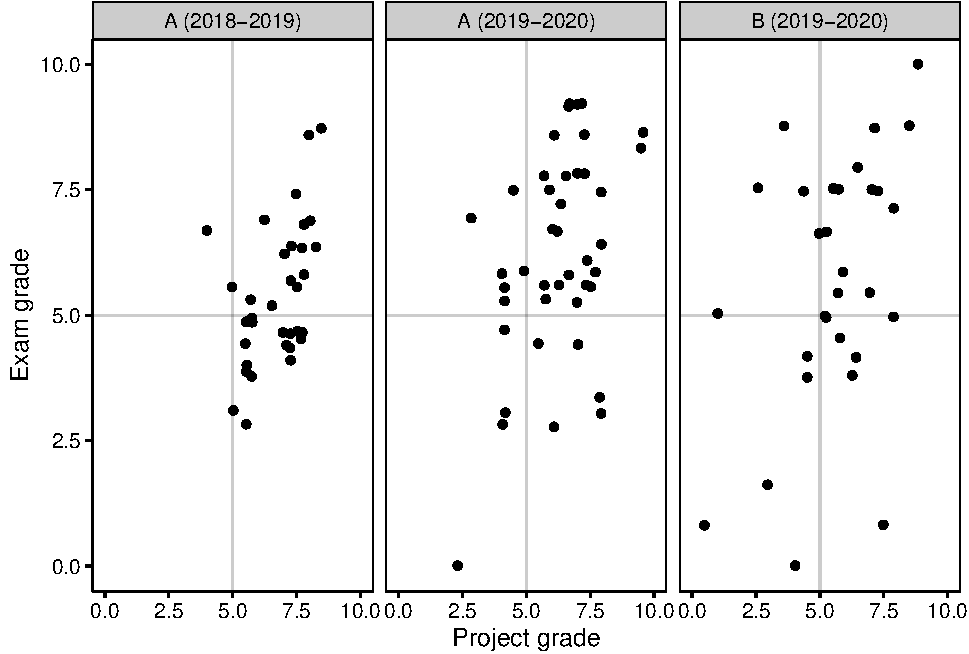
\includegraphics{teaching_data_science_files/figure-latex/unnamed-chunk-3-1.pdf}

The comparison of the marks obtained between the project and the exam
mark shows a strong disparity between these two types of evaluation.

The 2018-2019 year is the first year of transition to data science
courses. Only one student failed the project, while almost one third of
the students failed their exams. The level of requirements is being
raised for the 2019-2020 academic year. The new expectations and the
introduction of evaluation grids to assess projects show a greater
disparity in students' grades.

Despite an examination that includes theoretical and practical
questions, this type of assessment does not assess a student's ability
to correctly process and analyse biological data.

Following these results and the monitoring of more precise exercises,
the examination is definitively abandoned for the 2020-2021 academic
year to be replaced by a continuous assessment.

\hypertarget{students-profiles}{%
\subsection{Students' profiles}\label{students-profiles}}

{[}TODO : Add SOM analyses, This analysis is stand by as we validate the
metrics{]}

\hypertarget{temporality-of-work}{%
\subsection{temporality of work}\label{temporality-of-work}}

{[}TODO : add analyse on the commit or h5P/learnr exercices to follow
the student{]}

\hypertarget{learnr-tutorials}{%
\subsection{Learnr tutorials}\label{learnr-tutorials}}

The learnr tutorials are an essential part of the learning method to
link theory and practice. The cognitive load required to perform
tutorials is studied via a NASA LTX questionnaire.

\begin{Shaded}
\begin{Highlighting}[]
\FunctionTok{c}\NormalTok{(}\StringTok{"A99Wa\_perception"}\NormalTok{, }\StringTok{"B99Wa\_perception"}\NormalTok{, }\StringTok{"C99Wb\_perception:perception"}\NormalTok{) }\SpecialCharTok{\%\textgreater{}\%}
\NormalTok{  purrr}\SpecialCharTok{::}\FunctionTok{map\_dfr}\NormalTok{(learnr\_feeling, }\AttributeTok{df =}\NormalTok{ wo, }\AttributeTok{label =} \StringTok{"Q4"}\NormalTok{) }\SpecialCharTok{\%\textgreater{}.\%}
  \FunctionTok{mutate}\NormalTok{(., }\AttributeTok{course =} \FunctionTok{substr}\NormalTok{(app, }\AttributeTok{start =} \DecValTok{1}\NormalTok{, }\AttributeTok{stop =} \DecValTok{1}\NormalTok{)) }\OtherTok{{-}\textgreater{}}\NormalTok{ learnr\_workload}

\NormalTok{learnr\_workload }\SpecialCharTok{\%\textgreater{}.\%}
  \FunctionTok{pivot\_longer}\NormalTok{(.,}\AttributeTok{cols =} \FunctionTok{c}\NormalTok{(mental, physical, time\_pressure, performance, effort, frustration),}
  \AttributeTok{names\_to =} \StringTok{"category"}\NormalTok{, }\AttributeTok{values\_to =} \StringTok{"grade"}\NormalTok{)  }\SpecialCharTok{\%\textgreater{}.\%}
  \FunctionTok{left\_join}\NormalTok{(., dplyr}\SpecialCharTok{::}\FunctionTok{distinct}\NormalTok{(courses, course,name), }\AttributeTok{by =} \StringTok{"course"}\NormalTok{)}\OtherTok{{-}\textgreater{}}\NormalTok{ workload}

\NormalTok{workload }\SpecialCharTok{\%\textgreater{}.\%}
  \FunctionTok{group\_by}\NormalTok{(., user, app, course) }\SpecialCharTok{\%\textgreater{}.\%}
  \CommentTok{\#filter(., user != "ECAYEO033") \%\textgreater{}.\%}
  \FunctionTok{summarise}\NormalTok{(., }\AttributeTok{rtlx =} \DecValTok{10}\SpecialCharTok{*}\FunctionTok{mean}\NormalTok{(grade)) }\OtherTok{{-}\textgreater{}}\NormalTok{ workload\_rtlx}

\FunctionTok{set.seed}\NormalTok{(}\DecValTok{222}\NormalTok{)}
\FunctionTok{chart}\NormalTok{(workload\_rtlx, rtlx }\SpecialCharTok{\textasciitilde{}}\NormalTok{ course) }\SpecialCharTok{+}
  \FunctionTok{geom\_boxplot}\NormalTok{(}\AttributeTok{fill =} \StringTok{"\#00BFC4"}\NormalTok{) }\SpecialCharTok{+}
  \FunctionTok{geom\_jitter}\NormalTok{(}\AttributeTok{alpha =} \FloatTok{0.5}\NormalTok{, }\AttributeTok{width =} \FloatTok{0.1}\NormalTok{) }\SpecialCharTok{+}
  \FunctionTok{labs}\NormalTok{(}\AttributeTok{y =} \StringTok{"RTLX"}\NormalTok{, }\AttributeTok{x =} \StringTok{"Course"}\NormalTok{) }\SpecialCharTok{+}
  \FunctionTok{stat\_summary}\NormalTok{(}\AttributeTok{fun.y=}\StringTok{"mean"}\NormalTok{, }\AttributeTok{color =} \StringTok{"red"}\NormalTok{)}\SpecialCharTok{+}
  \FunctionTok{stat\_summary}\NormalTok{(}\AttributeTok{fun.data =}\NormalTok{ n\_fun, }\AttributeTok{geom =} \StringTok{"text"}\NormalTok{, }\AttributeTok{hjust =} \FloatTok{0.5}\NormalTok{) }\SpecialCharTok{+}
  \FunctionTok{labs}\NormalTok{( }\AttributeTok{y =} \StringTok{"Raw Task Load indeX (2020{-}2021)"}\NormalTok{)}
\end{Highlighting}
\end{Shaded}

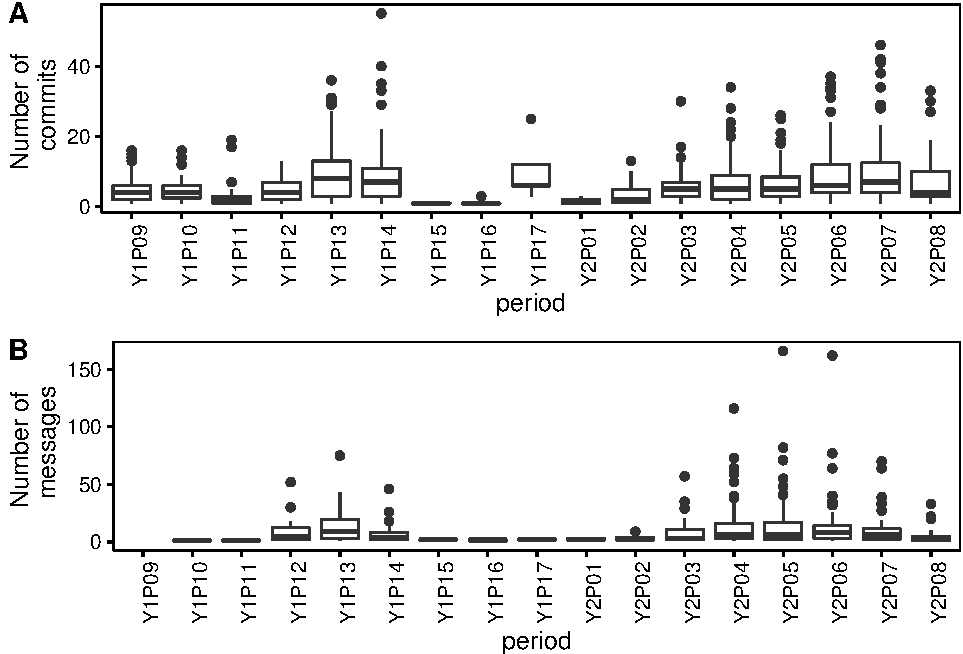
\includegraphics{teaching_data_science_files/figure-latex/unnamed-chunk-4-1.pdf}

The difficulty of the tutorial exercises increases from course to
course. However, we observe a significantly lower RTLX value for the
course C than for the course A (Tukey HSD, p-value = 0.023). The
cognitive load perceived by the students is therefore lower.

\begin{Shaded}
\begin{Highlighting}[]
\NormalTok{workload\_rtlx }\SpecialCharTok{\%\textgreater{}.\%}
  \FunctionTok{mutate}\NormalTok{(., }\AttributeTok{course =} \FunctionTok{as.factor}\NormalTok{(course)) }\OtherTok{{-}\textgreater{}}\NormalTok{ workload\_rtlx}

\CommentTok{\#kruskal.test(data = workload\_rtlx, rtlx \textasciitilde{} course)}
\CommentTok{\#summary(kw\_comp. \textless{}{-} nparcomp::nparcomp(data = workload\_rtlx, rtlx \textasciitilde{} course))}

\NormalTok{anova. }\OtherTok{\textless{}{-}} \FunctionTok{lm}\NormalTok{(}\AttributeTok{data =}\NormalTok{ workload\_rtlx, rtlx }\SpecialCharTok{\textasciitilde{}}\NormalTok{ course)}
\FunctionTok{anova}\NormalTok{(anova.)}
\end{Highlighting}
\end{Shaded}

\begin{verbatim}
## Analysis of Variance Table
## 
## Response: rtlx
##           Df  Sum Sq Mean Sq F value  Pr(>F)  
## course     2   926.9  463.47  3.5883 0.03134 *
## Residuals 98 12658.0  129.16                  
## ---
## Signif. codes:  0 '***' 0.001 '**' 0.01 '*' 0.05 '.' 0.1 ' ' 1
\end{verbatim}

\begin{Shaded}
\begin{Highlighting}[]
\CommentTok{\#bartlett.test(data = workload\_rtlx, rtlx \textasciitilde{} course)}
\CommentTok{\#plot(anova., which = 2)}

\FunctionTok{summary}\NormalTok{(anovaComp. }\OtherTok{\textless{}{-}} \FunctionTok{confint}\NormalTok{(multcomp}\SpecialCharTok{::}\FunctionTok{glht}\NormalTok{(anova.,}
  \AttributeTok{linfct =}\NormalTok{ multcomp}\SpecialCharTok{::}\FunctionTok{mcp}\NormalTok{(}\AttributeTok{course =} \StringTok{"Tukey"}\NormalTok{))))}
\end{Highlighting}
\end{Shaded}

\begin{verbatim}
## 
##   Simultaneous Tests for General Linear Hypotheses
## 
## Multiple Comparisons of Means: Tukey Contrasts
## 
## 
## Fit: lm(formula = rtlx ~ course, data = workload_rtlx)
## 
## Linear Hypotheses:
##            Estimate Std. Error t value Pr(>|t|)  
## A - B == 0    2.356      2.526   0.933   0.6183  
## C - B == 0   -6.058      3.296  -1.838   0.1607  
## C - A == 0   -8.414      3.141  -2.679   0.0229 *
## ---
## Signif. codes:  0 '***' 0.001 '**' 0.01 '*' 0.05 '.' 0.1 ' ' 1
## (Adjusted p values reported -- single-step method)
\end{verbatim}

\hypertarget{discussion}{%
\section{Discussion}\label{discussion}}

Les études portant sur le changements d'attitudes au sein de semestre ne
montre pas différence significative. La comparaison entre les 3 cours
met en avant qu'il faut plusieurs cours en continue afin d'observer une
chagement de la charge cognitive des étudiants.

apprentissage en continu sur 3 années successives (cohérence entre le
programme et l'approche pédagogique), les résultats sont meilleurs vers
la 3ieme années.

\hypertarget{conclusions}{%
\section{Conclusions}\label{conclusions}}

\begin{itemize}
\item
  Exam classique évalue mal la capacité d'evaluer des données
  biologiques par eux même
\item
  Les biologistes non expert de l'informatique est une challenge vu le
  nombre important de notions a apprendre utilisation d'un ordi, gestion
  de projet, statistique. Il faut décomposer ces notions en 5
  quadrimestre continue
\item
  Le logiciel reste vu comme pointu et diffficile d'utilisation (SUS).
\item
  l'evaluation continue et l'analyse de projet via des grilles critérié
  semble une approche intéressante pour juger de la capacité des
  étudiant à bosser.
\item
  la catégorisation des étudiants démontre une grande diversité de
  profils. Premier élément vers une pédagogie différencié vers
\end{itemize}

\hypertarget{references}{%
\section*{References}\label{references}}
\addcontentsline{toc}{section}{References}

\hypertarget{refs}{}
\begin{CSLReferences}{1}{0}
\leavevmode\hypertarget{ref-Auker2020}{}%
Auker, Linda A., and Erika L. Barthelmess. 2020. {``{Teaching R in the
undergraduate ecology classroom: approaches, lessons learned, and
recommendations}.''} \emph{Ecosphere} 11 (4): e03060.
https://doi.org/\url{https://doi.org/10.1002/ecs2.3060}.

\leavevmode\hypertarget{ref-Baker2016}{}%
Baker, Monya. 2016. {``1,500 Scientists Lift the Lid on
Reproducibility.''} \emph{Nature} 533 (7604): 452--54.
\url{https://doi.org/10.1038/533452a}.

\leavevmode\hypertarget{ref-Banks2019}{}%
Banks, George C., James G. Field, Frederick L. Oswald, Ernest H.
O'Boyle, Ronald S. Landis, Deborah E. Rupp, and Steven G. Rogelberg.
2019. {``{Answers to 18 Questions About Open Science Practices}.''}
\emph{Journal of Business and Psychology} 34 (3): 257--70.
\url{https://doi.org/10.1007/s10869-018-9547-8}.

\leavevmode\hypertarget{ref-Baumer2014}{}%
Baumer, Ben, Mine Cetinkaya-Rundel, Andrew Bray, Linda Loi, and Nicholas
J. Horton. 2014. {``{R Markdown: Integrating A Reproducible Analysis
Tool into Introductory Statistics}.''} \emph{Technology Innovations in
Statistics Education} 8 (1). \url{https://doi.org/10.5070/t581020118}.

\leavevmode\hypertarget{ref-Byers1989}{}%
Byers, J C, A Bittner, and S Hill. 1989. {``{Traditional and raw task
load index (TLX) correlations: Are paired comparisons necessary? In
A}.''} In.

\leavevmode\hypertarget{ref-Cetinkaya-Rundel2021}{}%
Çetinkaya-Rundel, Mine, and Victoria Ellison. 2021. {``{A Fresh Look at
Introductory Data Science}.''} \emph{Journal of Statistics and Data
Science Education} 29 (sup1): S16--26.
\url{https://doi.org/10.1080/10691898.2020.1804497}.

\leavevmode\hypertarget{ref-Cetinkaya-Rundel2018}{}%
Çetinkaya-Rundel, Mine, and Colin Rundel. 2018. {``{Infrastructure and
Tools for Teaching Computing Throughout the Statistical Curriculum}.''}
\emph{American Statistician} 72 (1): 58--65.
\url{https://doi.org/10.1080/00031305.2017.1397549}.

\leavevmode\hypertarget{ref-Donoho2017}{}%
Donoho, David. 2017. {``{50 Years of Data Science}.''} \emph{Journal of
Computational and Graphical Statistics} 26 (4): 745--66.
\url{https://doi.org/10.1080/10618600.2017.1384734}.

\leavevmode\hypertarget{ref-Estrellado2020}{}%
Estrellado, Ryan A., Emily A. Bovee, Jesse Mostipak, Joshua M.
Rosenberg, and Isabella C. Velásquez. 2020. \emph{{Data science in
education using R}}. London, England: Routledge.
\url{https://datascienceineducation.com/}.

\leavevmode\hypertarget{ref-Fiksel2019}{}%
Fiksel, Jacob, Leah R. Jager, Johannna S. Johanna S Hardin, and Margaret
A. Taub. 2019. {``{Using GitHub Classroom To Teach Statistics}.''}
\emph{Journal of Statistics Education} 27 (2): 110--19.
\url{https://doi.org/10.1080/10691898.2019.1617089}.

\leavevmode\hypertarget{ref-Freeman2014}{}%
Freeman, Scott, Sarah L. Eddy, Miles McDonough, Michelle K. Smith,
Nnadozie Okoroafor, Hannah Jordt, and Mary Pat Wenderoth. 2014.
{``{Active learning increases student performance in science,
engineering, and mathematics}.''} \emph{Proceedings of the National
Academy of Sciences of the United States of America} 111 (23): 8410--15.
\url{https://doi.org/10.1073/pnas.1319030111}.

\leavevmode\hypertarget{ref-Hart1988}{}%
Hart, Sandra G., and Lowell E. Staveland. 1988. {``{Development of
NASA-TLX (Task Load Index): Results of Empirical and Theoretical
Research}.''} \emph{Advances in Psychology} 52 (C): 139--83.
\url{https://doi.org/10.1016/S0166-4115(08)62386-9}.

\leavevmode\hypertarget{ref-Hsing2019}{}%
Hsing, Courtney, and Vanessa Gennarelli. 2019. {``{Using GitHub in the
Classroom Predicts Student Learning Outcomes and Classroom Experiences:
Findings from a Survey of Students and Teachers}.''} In
\emph{Proceedings of the 50th ACM Technical Symposium on Computer
Science Education}, 672--78. SIGCSE '19. New York, NY, USA: Association
for Computing Machinery. \url{https://doi.org/10.1145/3287324.3287460}.

\leavevmode\hypertarget{ref-Krathwohl2002}{}%
Krathwohl, David R. 2002. {``{A Revision of Bloom's Taxonomy: An
Overview}.''} \emph{Theory Into Practice} 41 (4): 212--18.
\url{https://doi.org/10.1207/s15430421tip4104_2}.

\leavevmode\hypertarget{ref-Larwin2011}{}%
Larwin, Karen, and David Larwin. 2011. {``{A Meta-Analysis Examining the
Impact of Computer-Assisted Instruction on Postsecondary Statistics
Education}.''} \emph{Journal of Research on Technology in Education} 43
(3): 253--78. \url{https://doi.org/10.1080/15391523.2011.10782572}.

\leavevmode\hypertarget{ref-Onwuegbuzie2003}{}%
Onwuegbuzie, Anthony J., and Vicki A. Wilson. 2003. {``{Statistics
Anxiety: Nature, etiology, antecedents, effects, and treatments--a
comprehensive review of the literature}.''} \emph{Teaching in Higher
Education} 8 (2): 195--209.
\url{https://doi.org/10.1080/1356251032000052447}.

\end{CSLReferences}

\end{document}
